\item \textbf{{[}ALVL/9597/2019/P2/Q2{]} }

Consider the following binary tree:
\begin{center}
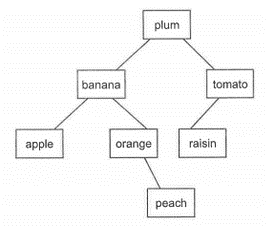
\includegraphics[width=0.35\paperwidth]{C:/Users/Admin/Desktop/Github/question_bank/LyX/static/img/9597-ALVL-2014-P2-Q2}
\par\end{center}
\begin{enumerate}
\item List the nodes, in order, that are visited for a post-order traversal.
\hfill{}{[}2{]}
\item List the nodes, in order, that are visited for an inorder traversal.
\hfill{}{[}2{]}
\item What property is exhibited by the list of items produced in \textbf{part
(b)}? \hfill{}{[}1{]}
\item Describe an algorithm, using pseudocode, to perform a binary tree
search. The output should state whether or not the item is present
in the tree. \hfill{}{[}5{]}
\end{enumerate}